\documentclass[]{article}
\usepackage{graphicx}
\usepackage{hyperref}
\usepackage{amsmath}
\usepackage{caption}
\usepackage{subcaption}
\usepackage{ngerman}
\usepackage[utf8]{inputenc}

%opening
\title{Balmer Series}
\author{Gunther T\"urk, Jonas Lehnen}

\begin{document}

\maketitle
\begin{abstract}
asdf

\end{abstract}

\tableofcontents

\newpage
\section{Theorie}
\subsection{Bohr Modell}
Der klassische Ansatz ein Atom zu beschreiben ist ungenügend. Normalerweise würde man ein durchgängiges Spektrum an Strahlung erwarten, da der Abstand zwischen Kern und Elektron zunächst nicht beschränkt ist. Das Gegenteil wird jedoch gemessen. Ebenso sollte von einer bewegten Ladung Strahlung emittiert werden, dies geschieht im Atom jedoch nur wenn sich der Abstand verkleinert. Dies bewegte Bohr 1913 dazu seine Postulate zu formulieren. Darin beschreibt er, dass das Elektron den Kern umkreist und durch die elektrostatische Kraft auf seiner Umlaufbahn gehalten wird ohne dabei Strahlung auszusenden. Diese Bahnen werden durch ihren Drehimpuls $l = pr = n\hbar$ beschrieben. Hier bei beschreibt $n$ die Ordnung der Bahn, auch Hauptquantenzahl genannt. Zuletzt entspricht die Energie des emittierten bzw. absorbierten Photons dem Energieunterschied des Elektrons auf verschiedenen Umlaufbahnen $ \hbar \omega = E_2 - E_1$. 

Generell erhält man aus der Behandlung der Schrödingergleichung dieselbe Energie für verschiedenen $n$, welche auch aus der Gleichsetzung von Coulomb- und Zentripetalkraft folgt. $R_\infty$ wird auch Rydbergkonstante genannt. 
\begin{equation}
E_n = -\frac{1}{2} m_0 c^2 \alpha^2 \frac{Z^2}{n^2} = -13.6eV \cdot \frac{Z^2}{n^2} \: ; \: \alpha = \frac{e^2}{4\pi\epsilon_0 \hbar c} = \frac{1}{137}
\end{equation}
\begin{equation}
\Delta E = R_\infty \left(\frac{1}{n^2} - \frac{1}{m^2} \right)  = -13.6eV \cdot \left(\frac{1}{n^2} - \frac{1}{m^2} \right)
\end{equation}
Dadurch können wir nun die Photonenenergie bestimmen, wenn ein Elektron seinen Bahn ändert. Im folgenden sowie bereits in der zweiten Gleichung behandeln wir das Wasserstoff Atom mit $Z=1$.Hierbei wird in verschiedene Serien unterschieden, je nachdem in welche das Elektron landet, nach Photon-Emission. Jede Serie wurde nach Entdecker benannt. Die ultravioletten Spektrallinien der Lyman (Ly) Serie $Ly_\alpha \:,\: Ly_\beta \:,\: Ly_\gamma \:,\: ...$ besitzt als Grundniveau den Zustand $n=1$. Analog wurden auch die infraroten Serien Brackett (B) $n=4$ und Paschen (Pa) $n=3$, sowie die sichtbare Balmer (H) Serie $n=2$ entdeckt. 
Die lateinische Nomenklatur beschreibt von wie vielen Niveaus oberhalb, auch states genannt, das Elektron auf das Endniveau gefallen ist. Die Anzahl wird mit den Buchstaben gleichgesetzt. So hei"st der \"Ubergang $5 \rightarrow 2$ auch $B_\gamma$.

\subsection{Ebert Monochromator}
Um das Licht eines Elements analysieren zu können müssen wir die Spektrallinien auffächern. Hier im Experiment wird dies mit einer Form des Ebert Monochromators umgesetzt. Dabei handelt es sich um um zwei  Spalte durch die das Licht ein- und ausfallen kann. Während dem Durchgang wird der Lichtstrahl zwischen zwei Reflexionen an einem Hohlspiegel auch an einem Gitter umgelenkt. Dieses Gitter ist nun drehbar und der Winkel $\delta$ in  Abbildung \ref{fig:Monochromator} bezeichnet die Verstellung bezüglich der parallel Lichtstrahlen. 

\begin{figure}[!h]
\centering
\begin{subfigure}{0.55\textwidth}
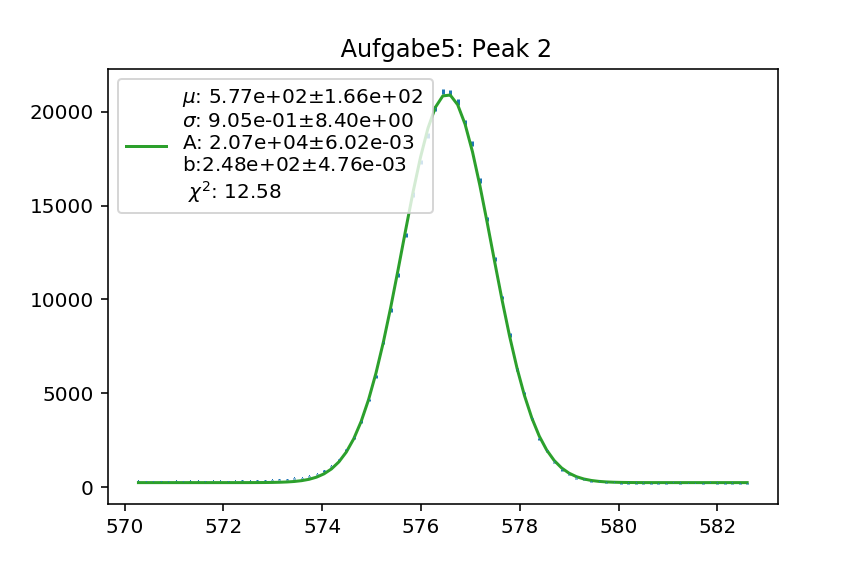
\includegraphics[width=\linewidth]{Plots/1.png}
\end{subfigure}
\begin{subfigure}[c]{0.4\linewidth}
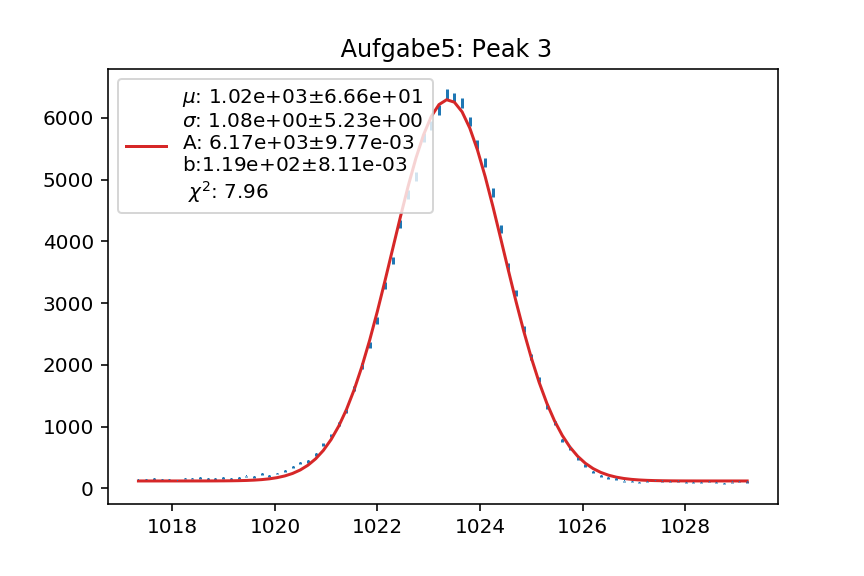
\includegraphics[width=\linewidth]{Plots/2.png}
\end{subfigure}
\caption{Schematische Darstellung eines Ebert Monochromators. Grafiken wurden dem zum Experiment mitgegebenen Skript (SS 2006) entnommen. }
\label{fig:Monochromator}
\end{figure}

Durch das drehbare Gitter erhält man trotz konstantem Strahlengang, welcher durch die festen Positionen der Spalte gegeben ist, eine Änderung im Laufweg des Lichts, je nach Wellenlänge. Diesen Unterschied erkennt man, wenn man wie im späteren Einzelspalt die verschiedenen Maxima betrachtet. 

% SKIZZE einfügen für den Strahlengang im Gitter + Herleitung
So erhält man aus Abbildung <<<ref>>> folgende Bedingung an Gangunterschied bei konstruktiver Interferenz:

\begin{equation}
\Delta = g\cdot sin(\beta) + g\cdot sin(\gamma) = g\cdot \left( sin(\delta - \alpha) + sin(\delta + \alpha)  \right)
\end{equation}
\begin{equation}
\Delta = g\cdot ( sin(\delta)cos(\alpha) + cos(\delta)sin(\alpha) +  sin(\delta)cos(\alpha) - cos(\delta)sin(\alpha) ) 
\end{equation}
\begin{equation}
\Delta= 2g \cdot cos(\alpha) sin(\delta) =: c \cdot sin(\delta) \stackrel{!}{=} n\lambda
\label{eq:}
\end{equation}
 
 

\subsection{Quantenmechanik}
\subsubsection{Schrödingergleichung}
Während das Bohrsche Atommodell in der Lage ist die Spektrallinien von Wasserstoff vorherzusagen, so versagt es doch bei der Erklärung der Fein- und Hyperfeinstruktur, sowie der Vorhersage von Spektrallinien bei Atomen mit mehr als einem Elektron. Aus der 1927 nachgewiesenen de Broglie Beziehung zwischen Impuls und Wellenlänge $ \lambda=\frac{h}{p} $ wobei h das Plank'sche Wikrungsquantum ist und der aus dem Photoeffekt bekannten Beziehung $ E=hf=\hbar \omega $ kann man die Schrödingergleichung motivieren. In der Quantenmechanik beschreibt man Teilchen mithilfe von Wellenfunktionen. Dabei beschreibt man ein freies Teilchen als ebene Welle.
\begin{equation}
\Psi(\vec{x},t)=A e^{i(k \vec{x}-\omega t)}
\end{equation} 
Als erstes betrachten wir die Zeit- und Ortsableitung dieser ebenen Welle. 
\begin{equation}
\label{eq:Energie} \frac{\partial}{\partial t} \Psi(\vec{x},t)=(-i\omega)  \Psi(\vec{x},t)=-\frac{iE}{\hbar} \Psi(\vec{x},t) \Rightarrow i\hbar \frac{\partial}{\partial t}=E  \Psi(\vec{x},t) \end{equation}
\begin{equation}
\label{eq:Impuls} \nabla  \Psi(\vec{x},t) =i\vec{k} \Psi(\vec{x},t)=\frac{i\vec{p}}{\hbar} \Psi(\vec{x},t) \Rightarrow -i\hbar \nabla  \Psi(\vec{x},t)= \vec{p}    \: \Psi(\vec{x},t) \end{equation}
Aus der klassischen Mechanik wissen wir, dass die Energie eines Teilchens \begin{equation} E=T+V=\frac{\vec{p}^2}{2\mu}+V(\vec{x}) 	\end{equation} wobei $\mu$ die reduzierte Masse ist. Um daraus eine quantenmechanische Beschreibung zu erhalten muss man den Impuls nach Gl. \ref{eq:Impuls} als $-i\hbar \nabla$ schhreiben und die Energie als $i \hbar \frac{\partial}{\partial t}$ schreiben und die Gleichung mit $\Psi(\vec{x},t)$ multiplizieren. Daraus erhält man dann 
\begin{equation}
\label{eq:Schrodinger}
i\hbar \frac{\partial}{\partial t}\Psi(\vec{x},t)=(-\frac{\hbar^2}{2\mu}\nabla^2+V(\vec{x})) \Psi(\vec{x},t) 
\end{equation}
was die Schrödingergleichung ist.
\subsubsection{Das Wasserstoffatom}
Um jetzt die gebundenen Energiezustände des Wasserstoffatoms zu berechnen und damit dann die $\delta E$ der Spektrallinien zu erhalten muss man die Schrödingergleichung für ein Potential
\begin{equation}
	V(r)=\frac{-e^2}{4\pi \epsilon} \frac{1}{r}
\end{equation}
lösen, also die Welleneigenfunkionen bestimmen. Da diese Rechnung in jedem Buch zur Quantenmechanik gefunden werden kann sparen wir uns hier die ausführlichen Rechnungen und Ergebnisse. Für unsere Zwecke reicht es zu wissen, dass die Energieniveaus $E_{n}$ gegeben sind durch
\begin{equation}
\label{eq:Wasserstoff}
	E_{n}=\frac{-e^4\mu}{8\epsilon_0^2h^2}*\frac{1}{n^2}=-\frac{\mu c^2}{2}\frac{\alpha^2}{n^2}
\end{equation} und wir aus der Lösung der Gleichung zwei weitere Quantenzahlen l,m erhalten, wobei l=0,1,2,...,n-1 den Drehimpuls quantifizieren und m=-l,(-l+1),...(l-1),l m die magnetische Quantenzahl ist. Die Energiewerte sind in l und m entartet, da diese die Energie für ein gegebenens n nicht ändern.
\subsubsection{Feinstruktur}
Die Entartung der Energiewerte aus Gl. \ref{eq:Wasserstoff} wird in l aufgehoben, wenn man die Korrekturen der Feinstruktur betrachetet. Dabei berücksichtigt man die relativistische Massenkorrektur des Elektrons sowie die Spin-Bahn-Kopplung des magnetischen Moments des Elektrons an seine Bahn. Außerdem kommt noch der Darwin-Term hinzu den man nicht durch Störungsrechnung motivieren kann, sondern ein Ergebnis der relativistischen Behandlung des Wasserstoffatoms mit der Dirac-Gleichung ist. 

%%Hier müssen die korrekturterme hin. und noch etwas beschriebung der LS kopplung 
%Na doppellinie"
\subsection{Beugung und Interferenz} %Neu schreiben mit es Photonen als anfang und dann welleneigenschaften
Interferenz und Beugung sind Phänomene die nur bei Wellen beobachtet werden. Die Überlegungen von de Broglie zur Materie-welle und der Beweis des Teilchencharakters von Photonen beschreiben die gleichzeitige Existenz eines Teilchens als Welle. Dies wird dann in der Quantenmechanik mathematisch Beschrieben. 
\subsubsection{Einfachspalt}
Fällt Licht auf einen einzelnen Spalt, so detektiert man dahinter nicht eine Normalverteilung der Intensität um die mitte des Spalts, sondern ein Interferenzmuster(Abb (\ref{fig:?????})). Insbesondere die Nebenmaxima lassen sich nicht mit klassischen Überlegungen erklären, da dieses Muster auch dann auftritt, wenn man einzelne Photonen durch den Spalt schickt und diese deshalb nicht miteinander Interferieren können.%Hier könnte man den klugscheißerkommentar anbringen vonwegen eichtheorie bla bla bla
Die Frage ist jetzt wie dieses Muster entstehen kann wo es doch nicht also Bewegung der Photonen aufgrund einer Bewegungsgleichung beschrieben wird. Betrachten wir das Photon als Teilchen, dass eine Wahrscheinlichkeitsdichte $\Psi(x)$ hat, dass sich auf den Spalt zubewegt, können wir es beschreiben als 
\begin{equation}
	Psi(x)=\Psi_{0}e^{i(kx-\omega t)}
\end{equation}
Der Einfachheit halber betrachten wir das Ganze nur in einer Dimension. Nach dem Fresnel'schen Prinzip entsteht an jedem Auftreffpunkt des Spalts eine neue Kugelwelle, welche bis auf eine eventuelle Phasenverschiebung von $\delta =y sin(\alpha) $ ihrer Ursprungswelle gleicht. Dabei ist zu beachten, dass eine Kugelwelle auch eine Beugung entgegen der Bewegungsrichtung des Strahls vorausgesetzt wird, die nicht beobachtet wird. Wir machen weiterhin die Annahme der Frauenhofer Beugung, d.h. dass sich der Schirm unendlich weit weg vom Spalt befindet. Die auslaufende welle kann also beschrieben werden als
\begin{equation}
	\Psi(x)=\Psi_{0}e^{i(k(x-\delta)-\omega t)}
\end{equation}
Auf einem unendlich weit entfernten Schirm treffen alle Strahlen die den Spalt parallel zueinander durchquert haben am selben Punkt auf. Um die Wahrscheinlichkeitsamplitude an diesem Punkt zu berechnen integrieren wir also über alle Wellen die den Spalt unter dem selben Winkel verlassen.
\begin{equation}%%%Hier muss irgendow noch ein psinull schlange hin, dass e^-ikx-wt mitnimmt
	\Psi_{Schirm}(x,\alpha)=\Psi_{0}e^{kx-\omega t}\dfrac{1}{d}\int_{-d/2}^{d/2} e^{-iky\: sin(\alpha)}
\end{equation}
\begin{equation}
	=-\frac{\Psi_{0}}{ikd \: sin \: \alpha} [e^{-iky \: sin(\alpha)}]^{+d/2}_{-d/2}
\end{equation}
\begin{equation}
	=-\frac{\Psi_{0}}{ikd \: sin \: \alpha} \underbrace{(e^{-ik\frac{d}{2}sin(\alpha)}-e^{ik\frac{d}{2}\:sin(\alpha)})}_{-2i\: sin(k\frac{d}{2}sin \alpha))}
\end{equation}
\begin{equation}
	=\Psi_{0}\frac{2}{kd\: sin \: \alpha}sin(\frac{\pi d}{\lambda}sin \: \alpha)
\end{equation}
Setzt man jetzt noch $k=\frac{2\pi}{\lambda}$ ein, so ergibt sich die relative Intensität zu
\begin{equation}
I_{relativ}=	\frac{|\Psi_{Schirm}|^2}{|\Psi_{0}|^2}=(\frac{\lambda}{\pi d \: sin \: \alpha} sin(\frac{\pi d}{\lambda} sin \: \alpha))^2
\end{equation}
\subsubsection{Doppelspalt}
Die Herleitung der Intensitätsverteilung beim Doppelspalt erfolgt analog zu der beim Einfachspalt. Anstatt aber nur über den einen Spalt zu integrieren, integriert man über zwei. 
%Hier das Bild vom Doppelspalt hin
\begin{equation}
	\Psi_{doppelt}(x,a)=\Psi_{0}\frac{1}{2d}(\int_{-D/2-d/2}^{-D/2+d/2}e^{-iky \: sin \: \alpha}dy+\int_{D/2-d/2}^{D/2+d/2}e^{-iky \: sin \: \alpha}dy)
\end{equation}
\begin{equation}
	=-\frac{\Psi_{0}}{2idk \: sin \: \alpha}([e^{-iky \: sin \alpha}]_{-D/2-d/2}^{-D/2+d/2}+[e^{-iky \: sin \alpha}]_{D/2-d/2}^{D/2+d/2})
\end{equation}


\begin{equation}
	=\frac{\Psi_{0}}{2idk \: sin \: \alpha}(e^{ik\frac{D}{2} sin \: \alpha}+ e^{-ik\frac{D}{2} sin \: \alpha})(e^{-ik\frac{d}{2} sin \: \alpha}+ e^{ik\frac{d}{2} sin \: \alpha})
\end{equation}

\begin{equation}
	=\Psi_{0}\frac{2}{dk \: sin \: \alpha}sin (\frac{kd}{2} sin \: \alpha)\: cos(\frac{kD}{2}sin \: \alpha)
\end{equation}
mit $k=\frac{2 \pi}{\lambda}$ ergibt sie die relative Intensität zu
\begin{equation}
	I_{relativ}=	\frac{|\Psi_{doppelt}|^2}{|\Psi_{0}|^2}=\left(\frac{\lambda}{\pi d \: sin \: \alpha}sin(\left  \frac{\pi d}{\lambda}sin \: \alpha \right)\right)^2 \cdot cos^2 \left( \frac{\pi D}{\lambda}sin \: \alpha \right) 
\end{equation}

%Hier muss dann die Herleitung hin
\subsubsection{Beugungsgitter}

\subsubsection{Balmer Serie}
\subsection{Isotopenshift}



(\subsection{Hyperfeinstruktur})
\subsection{Auswahlregeln} % (Vllt zur Balmerserie dazu)


\newpage
\section{Experiment}
\subsection{Setup}

Hier im Expermient wird ein Ebert Monochromator benutzt wie er auch schon in der Theorie beschrieben wurde. Der Aufbau wurde durch einen justierbaren Spiegel über dem Gitter erweitert. Der Spiegel ist verbunden mit der Gitterachse und dreht sich somit mit wenn der Winkel verändert wird. Dadurch wird zusätzliches Licht, das auf den Spiegel geworfen wird auf ein Maßband reflektiert. Dieses Maßband wurde in einem $90^\circ$ Winkel angebracht. Der Abstand zwischen Spiegel und Maßband wurde folgendermaßen ermittelt:

\begin{table}[h!]
	\centering
	\begin{tabular}{c|c|c|c|c|c}
		Messung & 1 & 2 & 3 & 4 & Mittelwert \\
		\hline
		Abstand [cm] & 250 & 250.5 & 250 & 250.5 & 250.25 $\pm$ 0.25 \\
	\end{tabular}
	\caption{Gemessene Abstände zwischen Spiegel und Maßband.}
\end{table}

%Wellenlängen der Na und Zi Lampe die wir zum kallibrieren verwendet haben:


\subsection{Auswertung}
\subsubsection{Gitterkonstante}
Die Gitterkonstante c ist essentiell für diesen Versuch, damit wir später die Rydbergkonstante bestimmen  können. Zunächst betrachten wir die theoretische Bestimmung von c.
%Tabelle
%Gemittelte Wellenlängen und energien der Übergänge
%Rydbergconstante
%Irgendwas mit den Dopplelinien
\subsection{Fehlerdiskussion}

\subsection{Fazit}

\section{Anhang}


\newpage
\begin{thebibliography}{}


\end{thebibliography}
\end{document}

